\chapter{Deep Learning for CT-Based Survival Analysis of Idiopathic Pulmonary Fibrosis Patients} \label{sec:deep_learning_for_ct_based_survival_analysis_of_idiopathic_pulmonary_fibrosis_patients_appendix}
    \newpage

    \section{Abstract} \label{sec:deep_learning_for_ct_based_survival_analysis_of_idiopathic_pulmonary_fibrosis_patients_appendix_abstract}
        \gls{IPF} is an \gls{ILD} that causes scarring of the lungs, leading to a decline in lung function and eventually death. Because this disease has a heterogeneous disease progression, predictive models could guide clinicians in making decisions about disease management. Some survival analysis methods, such as Cox, seek to rank participants based on their predicted survivability. However, Cox cannot directly output a survival time. DeepHit is a \gls{NN} based survival analysis method which predicts the most likely histogram bin of survival time. A disadvantage of DeepHit is that, when training, an error of one year is equivalent to an error of one hundred years. A common problem encountered is that training data is often censored, where the exact time of death is unknown except that it is past a censoring time. Here, a comparison of \gls{NN} approaches utilising five different losses is presented. Compared are ranking based approaches (such as Cox or Cox with a memory bank of previous predictions) and death distribution based approaches (such as DeepHit and likelihood with a uniform or Gaussian distribution to sample censoring times). The input to each model is a single \gls{CT} volume (plus optionally \gls{CF}) and the output is a survival time. Improvements over previous work include a larger model with a learned downsampling, a parameterised activation (which starts linear and becomes non-linear), a softplus output, orthogonal initialisation, an optimiser integrating weight decay, gradient accumulation, and an annealed learning rate. Evaluations used include \gls{MAE} and \gls{RAE}, the concordance index, the Brier score, and a visual analysis of \gls{Grad-CAM} results. Overall, the likelihood models performed the best, with DeepHit a close second and both Cox models a distant last. The \gls{EC} Likelihood model performed marginally better than the alternative.

    \section{Introduction} \label{sec:deep_learning_for_ct_based_survival_analysis_of_idiopathic_pulmonary_fibrosis_patients_appendix_introduction}
        Under the umbrella of \glspl{ILD}, \gls{IPF} is  characterised by a buildup of scar tissue in and a stiffening of the lungs of the patient. This leads to a reduction in the volume of the lung, resulting in a shortness of breath and eventually death. As with many other \glspl{ILD}, the progression of the disease is heterogeneous, and prognosis is challenging~\parencite{King2011IdiopathicFibrosis}.
        
        Previously, methods to monitor \gls{IPF} included testing lung function, with spirometric measurement of lung volume~\parencite{Watters1986AFibrosis}, or taking \gls{CT} acquisitions over time~\parencite{Lynch2018DiagnosticPaper}. Both approaches are limited by several factors, including, physical limitations of the patient, technical accuracy (spirometer baseline drift bias), and  longitudinal data availability. In contrast, measuring how long an \gls{IPF} patient could survive on the basis of a baseline \gls{CT} scan can be a useful clinical outcome to measure in order to prioritise resources and plan intervention. Furthermore, for research, it would be useful to accurately predict survival time in order to perform analysis of the disease itself. For this reason, here the focus is on accurately predicting \gls{IPF} patient death time based on a baseline \gls{CT} scan and associated \gls{CF}.
    
        In Cox Proportional Hazards Survival Analysis~\parencite{Cox1972RegressionLife-Tables} the death time of one participant is compared to another, and the model ranks patients according to their expected death times. However, a limitation is that the model does not directly output survival times. Recently models have been introduced that attempt to predict more directly the death time of a participant. For instance, DeepHit uses a \gls{CNN} to perform feature extraction on input \gls{CT} and outputs the probability of a survival time falling within predetermined bins of a death time histogram~\parencite{Lee2018DeepHit:Risks}. This treats survival analysis as a multi-class classification problem with a class for each time-bin that a patient could die in. A disadvantage is that the bins are not ordinally related and the model is penalised as much for making an error of one month as it is an error of ten years.
    
        Censoring is a significant issue in survival analysis in which the precise death time of a patient is unknown. For example, it may be known only that the patient is still alive, or that the patient died only within a specific time interval. In the \gls{OSIC} \gls{IPF} data set~\parencite{OSICOSICRepository}, approximately \SI{66}{\percent} of the records are right-censored, meaning that the time of death is above a known value but it is unknown by how much. A simple approach would be to remove censored data, however, this would discard a very significant fraction of training data. Missing data in clinical records is a related issue. Again, with approximately \SI{66}{\percent} of the \gls{OSIC} \gls{IPF} data~\parencite{OSICOSICRepository} set has some missing clinical information.
    
        Here, a number of survival analysis models that predict death time using a \gls{NN} are presented. The inputs of which being a baseline \gls{CT} scan and associated patient clinical information (such as height, age, etc). The models are able to address censoring and missing clinical information following~\parencite{Shahin2023DeepAnalysis, Shahin2022SurvivalData} respectively. Different training losses are used, including ones based on classical Cox based ranking, likelihood, and DeepHit. In the case of the Cox based loss, one with and one without a memory bank of previous predictions is used (to allow the loss to be approximated at all previously seen data points~\parencite{Shahin2022SurvivalData}). In the case of the likelihood based loss, one where censoring time is sampled in the classical way and one where censoring time is sampled from a uniform distribution is used~\parencite{Shahin2023DeepAnalysis}. Extensions over previous work include a change to the \gls{NN} architecture (larger, with a learnt downsampling, parameterised activation and softplus output, and orthogonal initialisation), a new optimiser, gradient accumulation (as such an increased batch size), and an annealed learning rate.
    
    \section{Methods} \label{sec:deep_learning_for_ct_based_survival_analysis_of_idiopathic_pulmonary_fibrosis_patients_appendix_methods}
        \subsection{Data Acquisition and Preparation} \label{sec:deep_learning_for_ct_based_survival_analysis_of_idiopathic_pulmonary_fibrosis_patients_appendix_data_acquisition_and_preparation}
            A total of $550$ \gls{CT} acquisitions were taken from the \gls{OSIC} data set~\parencite{OSICOSICRepository}. Each volume was segmented to remove data outside of the lung and was normalised independently. Where appropriate, \gls{CF}, such as age and sex were also used. If missing \gls{CF} were present, their value was imputed following~\parencite{Shahin2022SurvivalData}. Data were split into train and test groups using five fold \gls{CV}.

        \subsection{Models} \label{sec:deep_learning_for_ct_based_survival_analysis_of_idiopathic_pulmonary_fibrosis_patients_appendix_methods_models}
            Each \gls{NN} consisted of seven \gls{CNN} blocks, within which were two convolutions with stride one and one with stride two. Each convolution had a kernel size of three and used an orthogonal activation~\parencite{Hu2020ProvableNetworks}. Between each layer there was a \gls{PReLU} activation~\parencite{He2015DelvingClassification}, initialised with $\alpha$ set to one (meaning the network begins linear and becomes more non-linear as training progresses). At each downsampling step, the number of channels doubled. Global average pooling and flattening layers were used before fully connected layers reduced the number of units until it equals the output size (by halving the number of units at each layer). When \gls{CF} were used, they were concatenated to the output of the flattening layer. A softplus activation was used at the output for numerical stability. The model architecture was selected using the \gls{EC} Likelihood loss.
    
            AdamW was used as the optimiser, with weight decay, to improve the convergence rate as well as to penalise against large weights and overfitting~\parencite{Loshchilov2019DecoupledRegularization}. The learning rate started close to zero and increased linearly to the target learning rate over the first one tenth of iterations, before reducing back to close to zero over the next nine tenths. For each loss calculation a batch size of four was used, this is because Cox loss requires a batch size greater than one (for the sake of comparison the same number was used for all losses). This was approximately increased to $32$ using gradient accumulation, meaning eight gradients were averaged together at each iteration. Because of the \gls{MB} the effective batch size of Cox \gls{MB} was greater.
    
            For comparison, five loss functions were trialed.
    
            \begin{itemize}
                \item \textbf{\gls{EC} Likelihood} - Maximise likelihood using a Gaussian to model the time of death, where the censoring time was sampled from a uniform distribution from time zero up to the death time~\parencite{Shahin2023DeepAnalysis}.
    
                \item \textbf{Likelihood} - Maximise likelihood using a Gaussian to model the time of death, where the censoring time was sampled from a Gaussian distribution parameterised by the censor time. This is one of the classical ways to handle censoring~\parencite{Lee2018DeepHit:Risks}.
    
                \item \textbf{Cox} - Cox Proportional Hazards~\parencite{Cox1972RegressionLife-Tables}.
    
                \item \textbf{Cox \gls{MB}} - Cox Proportional Hazards with \gls{MB}~\parencite{Shahin2022SurvivalData}.
    
                \item \textbf{DeepHit} - Log-likelihood, with a maximum output value of $105$ years and $840$ bins~\parencite{Lee2018DeepHit:Risks}.
            \end{itemize}
    
            For both likelihood losses a fixed \gls{STD} equal to one year was used. For both Cox losses the output was converted to survival times using the Breslow estimator~\parencite{Breslow1974CovarianceData}.

        \subsection{Evaluation} \label{sec:deep_learning_for_ct_based_survival_analysis_of_idiopathic_pulmonary_fibrosis_patients_appendix_methods_evaluation}
            For evaluation of the results of the five loss functions the following methods were used. The \gls{MAE} and \gls{RAE} for the uncensored data between the predicted and true value was taken, the concordance index, the Brier score and a visual analysis of \gls{Grad-CAM} images~\parencite{Raykar2008OnIndex, Gerds2006ConsistentTimes, Selvaraju2020Grad-CAM:Localization}. For display of \gls{Grad-CAM} a slice was selected which displayed fibrosis in the base of both lungs. Only the model without \gls{CF} was used for \gls{Grad-CAM} extraction.
    
    \section{Results} \label{sec:deep_learning_for_ct_based_survival_analysis_of_idiopathic_pulmonary_fibrosis_patients_appendix_results}
        \begin{table}
            \centering
            
            \captionsetup{singlelinecheck=false}
            \caption{
                A comparison of \gls{MAE}, \gls{RAE}, the concordance index, and the Brier score. The average survival time was approximately $32$ months.
            }
            
            \resizebox*{1.0\linewidth}{!}
            {
                \begin{tabular}{||c|cc|c|c||}
                    \hline
                                                            & \textbf{\gls{MAE}} & \textbf{\gls{RAE}} & \textbf{C-Index}  & \textbf{Brier}    \\
                    \hline
                    \textbf{\gls{EC} Likelihood}            & $22.7\pm1.51$      & $1.72\pm0.89$      & $0.77\pm0.05$     & $0.22\pm0.07$      \\
                    \textbf{\gls{EC} Likelihood \gls{CF}}   & $21.5\pm1.32$      & $1.98\pm0.82$      & $0.80\pm0.03$     & $0.18\pm0.05$      \\
                    \textbf{Likelihood}                    & $28.9\pm1.96$      & $2.23\pm0.01$      & $0.76\pm0.05$     & $0.25\pm0.01$      \\
                    \textbf{Likelihood \gls{CF}}           & $25.3\pm1.74$      & $2.04\pm0.01$      & $0.75\pm0.04$     & $0.20\pm0.01$      \\
                    \hline
                    \textbf{Cox}                           & $187 \pm309 $      & $17.0\pm30.7$      & $0.73\pm0.04$     & $0.61\pm0.28$      \\
                    \textbf{Cox \gls{CF}}                  & $233 \pm287 $      & $26.4\pm21.9$      & $0.72\pm0.03$     & $0.57\pm0.16$      \\
                    \textbf{Cox \gls{MB}}                  & $166 \pm267 $      & $17.7\pm28.2$      & $0.74\pm0.03$     & $0.53\pm0.31$      \\
                    \textbf{Cox \gls{MB} \gls{CF}}         & $179 \pm294 $      & $16.3\pm22.8$      & $0.73\pm0.05$     & $0.56\pm0.24$      \\
                    \hline
                    \textbf{DeepHit}                       & $38.4\pm14.8$      & $3.99\pm0.34$      & $0.72\pm0.03$     & $0.40\pm0.01$      \\
                    \textbf{DeepHit \gls{CF}}              & $31.3\pm9.19$      & $3.50\pm0.42$      & $0.71\pm0.04$     & $0.42\pm0.01$      \\
                    \hline
                \end{tabular}
            }
            \label{tab:deep_learning_for_ct_based_survival_analysis_of_idiopathic_pulmonary_fibrosis_patients_appendix_results_table}
        \end{table}
    
        \begin{figure}\centering
    
            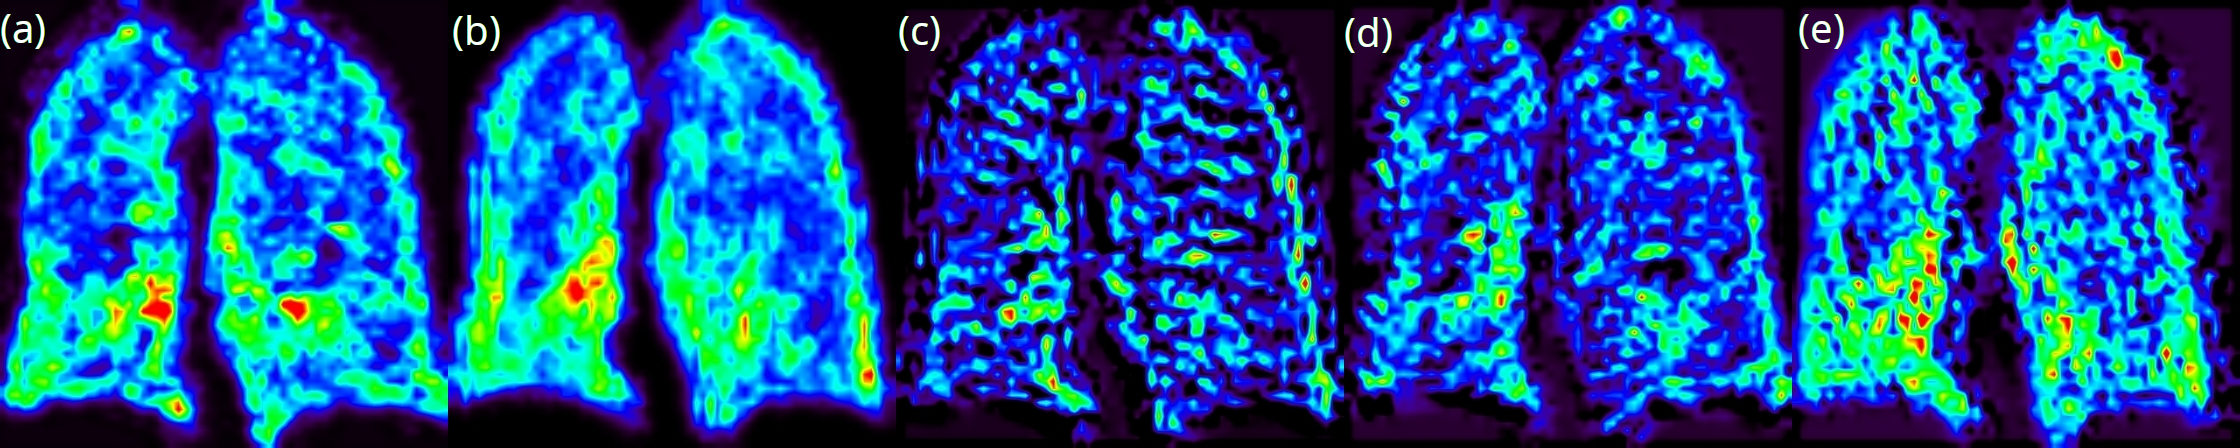
\includegraphics[width=1.0\linewidth]{figures/survival_analysis_grad_cam_label.png}
            
            \captionsetup{singlelinecheck=false}
            \caption{
                From left to right a slice through a fibrotic region of a \gls{Grad-CAM} image, taken from a middle convolution, of a $65$ year old patient with a survival time of $30$ months for (a) Death Conditional Likelihood, (b) Likelihood, (c) Cox, (d) Cox \gls{MB}, and (e) DeepHit. All colour maps are consistent for all images.
            }
            \label{fig:deep_learning_for_ct_based_survival_analysis_of_idiopathic_pulmonary_fibrosis_patients_appendix_results_grad_cam}
       \end{figure}
    
        From~\Fref{tab:deep_learning_for_ct_based_survival_analysis_of_idiopathic_pulmonary_fibrosis_patients_appendix_results_table} it can be seen that the the \gls{MAE} and \gls{RAE} are often lower for both likelihood based models than for all other models. The \gls{MAE} and \gls{RAE} for the DeepHit model is lower than that of the Cox based model, while for the Cox based models not only are their errors high but they also have a substantially higher variance. The \gls{MAE} and \gls{RAE} of the \gls{EC} Likelihood model is often lower than that of the Likelihood model. The Brier score results also back up this assertion, however it is difficult to draw conclusions from the concordance index results. The results also seem to indicate that there is some benefit to including the \gls{CF}, although from these results alone it is not possible to say if this is due to the added information from the \gls{CF} or the increase in model size. From~\Fref{fig:deep_learning_for_ct_based_survival_analysis_of_idiopathic_pulmonary_fibrosis_patients_appendix_results_grad_cam} it can be seen that both likelihood based model and DeepHit produced updates which identified the fibrosis in both lungs, the Cox based model only seemed to detect fibrosis in the left lung. Both likelihood models seemed to extract updates which are less noisy than the DeepHit update.
    
    \section{Discussion and Conclusions} \label{sec:deep_learning_for_ct_based_survival_analysis_of_idiopathic_pulmonary_fibrosis_patients_appendix_discussion_and_conclusions}
        From a comparison of errors and a visual analysis it appears that the likelihood based models provide the best results most often.
        
        The model used for the DeepHit model had more parameters than the model used for all other methods (due to the output being larger), thus it may not be an entirely fair comparison. However, while using a larger model the method does not provide results significantly better than the likelihood models.
        
        When \gls{CF} were used it seems to improve results, although not significantly. For the increase in complexity it may not be worth including.
        
        What is not factored into the results is computation time. The Cox loss without \gls{MB} is the fastest to compute, the likelihood losses are not much longer. The DeepHit loss takes slightly longer than both previous methods while the Cox \gls{MB} loss takes magnitudes longer (approximately six hours vs four days).
    
        In the future it may be interesting to take the survival time output from the models presented here and use them as part of a generative model to predict \gls{CT} acquisitions with a lower survival time.
    